%!TEX TS-program = xelatex
\documentclass[]{friggeri-cv}
\usepackage{afterpage}
\usepackage{hyperref}
\usepackage{color}
\usepackage{xcolor}
\hypersetup{
    pdftitle={},
    pdfauthor={},
    pdfsubject={},
    pdfkeywords={},
    colorlinks=false,       % no lik border color
   allbordercolors=white    % white border color for all
}
\RequirePackage{xcolor}
\definecolor{pblue}{HTML}{0395DE}

\usepackage{enumitem}

\begin{document}
\header{Victor M.}{Mendiola-Lau}{Científico de la Computación, Investigador e Ingeniero de Software}
      
% Fake text to add separator      
\fcolorbox{white}{gray}{\parbox{\dimexpr\textwidth-2\fboxsep-2\fboxrule}{%
.....
}}

% In the aside, each new line forces a line break
\begin{aside}
  \section{Dirección}
    Jaén, Jaén, España
    ~
    ~
    ~
  \section{Teléfono}
    (+34) 621 06 15 01
    ~
    ~
    ~
  \section{Correo}
    \href{mailto:ryuzakyl@gmail.com}{\textbf{ryuzakyl@}gmail.com}
	~
	~    
    ~
  \section{Perfiles web}
    \href{https://github.com/ryuzakyl}{{\scriptsize github.com/ryuzakyl}}
    \href{https://independent.academia.edu/VictorMendiolaLau}{{\scriptsize academia.edu/VictorMendiolaLau}}
    \href{https://www.linkedin.com/in/VictorMendiolaLau}{{\scriptsize linkedin.com/in/VictorMendiolaLau}}
	\href{https://www.researchgate.net/profile/Victor_Mendiola-Lau}{{\scriptsize researchgate.net/Victor\char`_Mendiola-Lau}}
    ~
    ~
    ~
  \section{Habilidades personales}
    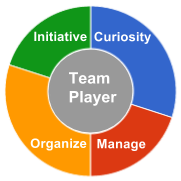
\includegraphics[scale=0.62]{img/personal.png}
    ~
%    ~
%  \section{Programming}
%    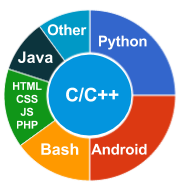
\includegraphics[scale=0.62]{img/programming.png}
%    ~
\end{aside}

\section{Ingeniería de Software}
\begin{entrylist}
  \entry
    {09/18 - Now}
    {Ingeniero de Software}
    {Kitsune Technologies, Tennessee, EUA}   
    {Amplia gama de responsabilidades, incluyendo Análisis de Datos, Visión por Computadora, Desarrollo Web, implementación de servicios, etc.\\}

  \entry
    {09/17 - 11/18}
    {Desarrollador Web Full Stack}
    {}
    {Aplicaciones web como soluciones al manejo de las fuerzas de trabajo. Tecnologías: PHP, HTML, CSS3, JavaScript, jQuery, MySQL, etc.\\}
    
  \entry
    {12/17 - 02/18}
    {Desarrollador de Backend en Python/Django}
    {SBY Technologies, Florida, EUA}
    {Desarrollo de un API desde cero con autenticación mediante JWT, generación automática de reportes (.pdf, .csv), etc. También desempeñé el rol de ingeniero de DevOps y Administrador de Sistemas en Linux.\\}
    
  \entry
    {02/16 - 03/16}
    {Desarrollador de Backend en Ruby/Rails}
    {Ksabes, La Habana, Cuba}
    {Diseño e implementación propia de un API basada en Json Web Token (JWT) para la autenticación.\\}

  \entry
    {09/14 - 01/15}
    {Desarrollador de Ruby}
    {IRStrat, México D.F., México}
    {Diseño e implementación propia de un servicio concurrente y multi-hilos para consumir información de la bolsa de valores en tiempo real.\\}

  \entry
    {09/13 - 09/17}
    {Ingeniero de Software}
    {CENATAV, La Habana, Cuba}
    {Desarrollador de Aplicaciones de Escritorio Full Stack en .NET Framework, específicamente en C\#. Diseño y desarrollo eficiente de algoritmos en C/C++. Integración de aplicaciones de escritorio en .NET con bibliotecas implementadas en C/C++ mediante PInvoke.\\}    
    
\end{entrylist}

\section{Investigación \& Docencia}
\begin{entrylist}
  \entry
    {09/18 - 12/18}
    {Investigador Visitante}
    {Universidad de Sevilla, España}
    {Investigador en temas de Aprendizaje de Máquina y Análisis de Datos.\\}
    
  \entry
    {10/17 - 09/18}
    {Profesor Instructor}
    {Universidad de La Habana, Cuba}
    {Instructor de Matemática en temáticas como Teoría de Conjuntos, Funciones, Álgebra, Cálculo, Matemática Numérica y Ecuaciones Diferenciales Ordinarias.\\}
  
  \entry
    {09/13 - 09/17}
    {Investigador}
    {CENATAV, La Habana, Cuba}
    {Diseño y desarrollo de Sistemas de Reconocimiento de Patrones. Investigador Júnior y estudiante de doctorado. Con intereses en temas como Aprendizaje de Máquina, Análisis de Datos, Representación de Datos y Visión por Computadoras. Tecnologías: Python, Numpy, SciPy, Matplotlib, scikit-learn, etc.\\}
\end{entrylist}


\begin{entrylist}
  \entry
    {06/12 - 07/12}
    {Pasantía de investigación}
    {CENATAV, La Habana, Cuba}
    {Diseño e implementación de un método para codificar el iris basado en el Análisis de Datos Funcionales (FDA).\\}

  \entry
    {09/10 - 06/13}
    {Instructor asistente}
    {Universidad de La Habana, Cuba}
    {Instructor  de Programación y Algoritmos para la carrera de Matemática en la Facultad de Matemática y Computación (MATCOM).\\}
\end{entrylist}

\section{Otras responsabilidades}
\begin{entrylist}
  \entry
    {11/18 - 10/19}
    {Consultor}
    {PNWA, Seattle, USA}
    {Miembro del grupo consultor Pacific NorthWest Advisors (PNWA) realizando estudios de mercado y de la informática dentro de Cuba y brindando también información única a las empresas del noroeste del Pacífico.}

\end{entrylist}

\section{Educación/Formación académica}
\begin{entrylist}
  \entry
    {2019 - }
    {Máster en Seguridad Informática}
    {Universidad de Jaén, España}
    {
    	Materias principales: Aplicaciones Seguras en la Nube, Seguridad en las Redes, Detección de Intrusiones, Ingeniería Inversa, Análisis de Malware, Criptografía Avanzada.\\
%    	\emph{Title of the Thesis: "A Handoff Algorithm based on Link Quality Prediction for Mass Transit Wireless Mesh Networks".}\\
%    	\emph{Relators: Prof. Enzo Mingozzi, Ing. Carlo Vallati, Prof. Luciano Lenzini.}\\
    }

  \entry
    {2008 - 2013}
    {B.Sc. en Ciencia de la Computación}
    {Universidad de La Habana, Cuba}
    {Título de Oro (5.13 de 5.0) en Ciencia de la Computación.\\ Materias principales: Programación, Estructuras de Datos y Algoritmos, Teoría de la Complejidad Computacional, Matemática, Investigación Operacional, Matemática Numérica e Inteligencia Artificial.\\
    \emph{Título de la Tesis: "Reconocimiento de iris utilizando Análisis de Datos Funcionales".}}

%  \entry
%    {2004 - 2007}
%    {Bachelor Diploma}
%    {IPVCE Vladimir Ilich Lenin, Havana, Cuba}
%    {Bachelor diploma with focus on these subjects: Matematics and Computer Science.}
\end{entrylist}

\section{Idiomas}
\begin{entrylist}
  \entry
    {\textbf{Español}}
    {}
    {}
    {Lengua materna}      

  \entry
    {\textbf{Inglés}}
    {}
    {}
    {
		\textbf{Usuario experto}: Puntuación del IELTS de 7.0 (nivel \textbf{C1} en el CEFR).\\    
    	Graduado \textbf{\emph{summa cum laude}} de la Escuela de Idiomas \emph{Abraham Lincoln}.
    }

  \entry
    {\textbf{Francés}}
    {}
    {}
    {Diploma de estudios de la Lengua Francesa (\textbf{DELF B2}).}
\end{entrylist}

\section{Certificados \& Cursos de formación}
\begin{entrylist}
  \entry
    {2014}
    {(Postgrado) Metodologías de la Investigación}
    {CENATAV, IDICT}
    {\emph{Desmitificar la investigación y los métodos de investigación. Bosquejo de los fundamentos de la investigación.}}
\end{entrylist}

\begin{entrylist}    
  \entry
    {2013}
    {(Tutorial) Fundamentos del Reconocimiento de Iris}
    {Congreso CIARP 2013}
    {\emph{Tutorial presentado por el Profesor Tieniu Tan sobre los avances y retos del Reconocimiento de Iris.}}

  \entry
    {}
    {(Tutorial) Análisis de grandes volúmenes de datos}
    {Congreso CIARP 2013}
    {\emph{Minería de datos inciertos y probabilísticos para grandes volúmenes de datos por el Profesor Jian Pei.}}
    
  \entry
    {}
    {(Licenciatura) \LaTeX}
    {Universidad de La Habana}
    {\emph{Introducción al lenguaje de descripción de documentos construido sobre \TeX.}}
\end{entrylist}
       
\begin{entrylist}
  \entry
    {2012}
    {(Postgrado) Estructuras de Datos Avanzadas}
    {Universidad de La Habana}
    {\emph{Introducción a conceptos como el Análisis amortizado, Heaps de Fibonacci, Splay Trees, etc.}}      

  \entry
    {}
    {(Licenciatura) Inteligencia de Negocios}
    {Universidad de La Habana}
    {\emph{Introducción a los conceptos fundamentales de los procesos modernos de Inteligencia de Negocios.}}

  \entry
    {}
    {(Licenciatura) Introducción a la Criptografía}
    {Universidad de La Habana}
    {\emph{Introducción a los conceptos fundamentales de la Criptografía moderna.}}
\end{entrylist}

\begin{entrylist}
  \entry
    {2011}
    {(Licenciatura) Introducción a la Visión por Computadora}
    {Universidad de La Habana}
    {\emph{Fundamentos de la Visión por Computadora con OpenCV.}}      

  \entry
    {}
    {(Licenciatura) Introducción a los Gráficos por Computadora}
    {Universidad de La Habana}
    {\emph{Fundamentos de los Gráficos por Computadora.}}
\end{entrylist}

\section{Tecnologías}
\begin{entrylist}
  \entry
    {\textbf{Lenguajes}}
    {}
    {}
    {\textbf{C\#} (+9 años), \textbf{Python} (+7 años), \textbf{C/C++} (+5 años), \textbf{Ruby} (+2 años), \textbf{PHP} (+2 años). Otros lenguajes incluyen \textbf{Go} y \textbf{Java}.}
\end{entrylist}

\begin{entrylist}
  \entry
    {\textbf{IDEs\&Editores}}
    {}
    {}
    {\textbf{Visual Studio}, \textbf{VS Code} e \textbf{IDEs de JetBrains}.}

  \entry
    {\textbf{ML \& DA}}
    {}
    {}
    {Tecnologías basadas en Python para el Aprendizaje de Máquina y el Análisis de Datos: \textbf{Numpy}, \textbf{SciPy}, \textbf{Pandas}, \textbf{scikit-learn} and \textbf{Matplotlib}. Además del lenguaje de programación y ambiente \textbf{MATLAB}.}

  \entry
    {\textbf{Web}}
    {}
    {}
    {\textbf{HTML}, \textbf{CSS3}, \textbf{JavaScript}, \textbf{Vue.js}, \textbf{jQuery}, \textbf{PHP}, \textbf{Django}, \textbf{Django Rest Framework}, \textbf{ASP.NET MVC/Core} y \textbf{Ruby on Rails}.}

  \entry
    {\textbf{Cloud}}
    {}
    {}
    {\textbf{AWS} y \textbf{Google Cloud Platform}.}

  \entry
    {\textbf{Desktop}}
    {}
    {}
    {\textbf{.NET}, \textbf{.NET Core} y \textbf{Qt}.}

  \entry
    {\textbf{DVCS}}
    {}
    {}
    {\textbf{Git} (+5 años) (\textbf{GitHub}, \textbf{GitLab} y \textbf{Bitbucket}).}
    
  \entry
    {\textbf{DBMS}}
    {}
    {}
    {\textbf{PostgreSQL}, \textbf{Microsoft SQL Server}, \textbf{MySQL} y \textbf{SQLite}.}
    
  \entry
    {\textbf{CV}}
    {}
    {}
    {\textbf{OpenCV}, \textbf{EmguCV} y \textbf{OpenCV-Python bindings}.}    

  \entry
    {\textbf{SO}}
    {}
    {}
    {\textbf{GNU/Linux} (+4 años) (\textbf{Ubuntu}, \textbf{Linux Mint}) y \textbf{Microsoft Windows} (+15 años).}
\end{entrylist}

\pagebreak

\section{Publicaciones}
\begin{paperlist}
  \paperentry
    {2017}
    {}
    {}
    {
		\emph{(Aceptada)} \textbf{Victor Mendiola-Lau}, Francisco J. Silva Mata, Yenisel Plasencia Calaña, Isneri Talavera Bustamante and Maria De Marsico. ``Bio-chemical Data Classification by Dissimilarity Representation and Template Selection." \emph{CIARP}, 2017.
    }
\end{paperlist}

\vspace{0.5cm}

\begin{paperlist}
  \paperentry
    {2016}
    {}
    {}
    {
		\textbf{Victor Mendiola-Lau}, F.J. Silva-Mata, Y. Martínez-Díaz, I. Talavera Bustamante and M. De Marsico. ``Exploratory Data Analysis Combined with Entropy-based Template Selection for the Identification of Mixed Substances."	 \emph{CAC}, 2016.
    }
\end{paperlist}

\begin{paperlist}
  \paperentry
    {}
    {}
    {}
    {
		\textbf{Victor Mendiola-Lau}, Francisco J. Silva Mata, Yoanna Martínez-Díaz, Isneri Talavera Bustamante, Maria De Marsico. ``Hierarchical Clustering Combined with Entropy Based-template Selection and SVM Classification for the Identification of Mixed Substances by Means of UV and GC Analytical Technique." \emph{Informática}, 2016.
    }
\end{paperlist}

\begin{paperlist}
  \paperentry
    {}
    {}
    {}
    {
		\textbf{Victor Mendiola-Lau}, Francisco J. Silva Mata, Yoanna Martínez-Díaz, Isneri Talavera Bustamante and Maria De Marsico. ``Automatic classification of herbal substances enhanced with an entropy criterion." \emph{CIARP}, 2016.
    }
\end{paperlist}

\vspace{0.5cm}

\begin{paperlist}
  \paperentry
    {2015}
    {}
    {}
    {
		Francisco J. Silva-Mata, \textbf{Victor Mendiola-Lau}, Isneri Talavera-Bustamante and Yoanna Martínez-Díaz. ``Automatic processing of TLC images for discovering clusters and performing classification tasks of herbal substances. Case of study". \emph{SSC14}, 2015.
    }
\end{paperlist}

\begin{paperlist}
  \paperentry
    {}
    {}
    {}
    {
		Francisco J. Silva Mata, Dania P.- Muñoz, Stefano Berretti, \textbf{Victor Mendiola-Lau}, Isneri Talavera Bustamante, Noslen Hernández, Yoanna Martínez-Díaz, Angel Augier . ``Alineación de señales e imágenes durante la aplicación del análisis de datos funcionales: Ejemplos prácticos en señales e imágenes quimiométricas y biométricas." \emph{RCF}, 2015.
    }
\end{paperlist}

\begin{paperlist}
  \paperentry
    {}
    {}
    {}
    {
		Francisco J. Silva Mata, Dania P.- Muñoz, \textbf{Victor Mendiola-Lau}, Isneri Talavera Bustamante, Angel Augier. ``Criterios y métodos de selección de bases y su impacto en el análisis de datos funcionales: Algunos ejemplos en biometría". \emph{RCF}, 2015.
    }
\end{paperlist}

\begin{paperlist}
  \paperentry
    {}
    {}
    {}
    {
		\textbf{Victor Mendiola-Lau}, Isneri Talavera Bustamante and Maria de Marsico. ``Clustering of simple and multi-way spectral data on the dissimilarity representation." \emph{Serie Azul CENATAV}, 2015.
    }
\end{paperlist}

\begin{paperlist}
  \paperentry
    {}
    {}
    {}
    {
		Francisco J. Silva Mata,  Isneri Talavera, \textbf{Victor Mendiola-Lau}, Yoanna Martínez Díaz, Anier Revilla Eng. ``Clasificación de Sustancias Vegetales con el uso de un Sistema Automatizado para el proceso de Imágenes de TLC". En: IX Congreso de Ciencias, Tecnología e Innovación Química, Quimicuba 2015, La Habana, Cuba, 13-16 de octubre de 2015.
    }
\end{paperlist}

\begin{paperlist}
  \paperentry
    {}
    {}
    {}
    {
		Dania Porro, Isneri Talavera, Robert Duin, Gabriela Barcas, \textbf{Victor Mendiola-Lau}. ``Comparación De Diferentes Formas De Representación De Datos Espectrales Para Clasificación De Sustancias." En: IX Congreso de Ciencias, Tecnología e Innovación Química, Quimicuba 2015, La Habana, Cuba, 13-16 de octubre de 2015.
    }
\end{paperlist}

\begin{paperlist}
  \paperentry
    {}
    {}
    {}
    {
		Francisco J. Silva Mata, \textbf{Victor Mendiola-Lau}, Anier Revilla, Isneri Talavera, Angel Augier, Stefano Berretti y Yoanna Martínez. Optimización de los Modelos Funcionales para Objetos Biométricos. \emph{RECPAT}, 2015.
    }
\end{paperlist}

\vspace{0.5cm}

\begin{paperlist}
  \paperentry
    {2014}
    {}
    {}
    {
		Francisco J. Silva-Mata, Dania P.-Muñoz, \textbf{Victor Mendiola-Lau}, Isneri Talavera-Bustamante, Angel Augier. ``Criteria and methods of selection of bases and their impact in functional data analysis. Some examples in biometrics". \emph{CIOFF}, 2014.
    }
\end{paperlist}

\begin{paperlist}
  \paperentry
    {}
    {}
    {}
    {
		Francisco J. Silva-Mata, Dania P.-Muñoz, Stefano Berretti, \textbf{Victor Mendiola-Lau}, Isneri Talavera-Bustamante, Noslen Hernández, Yoanna Martínez-Díaz, Angel Augier. ``Signal and image alignment during the application of functional data analysis. Practical examples of chemometrics and biometrics". \emph{CIOFF}, 2014.
    }
\end{paperlist}

\begin{paperlist}
  \paperentry
    {}
    {}
    {}
    {
		\textbf{Victor Mendiola-Lau}, Francisco J. Silva-Mata, Dania P.-Muñoz, Isneri Talavera-Bustamante. ``APIris: Nueva Plataforma Automatizada para el Reconocimiento de Iris". \emph{RECPAT}, 2014.
    }
\end{paperlist}

\begin{paperlist}
  \paperentry
    {}
    {}
    {}
    {
		Francisco J. Silva-Mata, Dania P.-Muñoz, \textbf{Victor Mendiola-Lau}, Anier Revilla-Eng, Isneri Talavera-Bustamante. ``Criterios y métodos para representar imágenes biométricas usando FDA". \emph{RECPAT}, 2014.
    }
\end{paperlist}

\vspace{0.5cm}

\begin{paperlist}
  \paperentry
    {2013}
    {}
    {}
    {
		Dania P.-Muñoz, Francisco J. Silva-Mata, \textbf{Victor Mendiola-Lau}, Noslen Hernández, and Isneri Talavera-Bustamante. ``A new iris recognition approach based on a functional representation". \emph{CIARP}, 2013.
    }
\end{paperlist}

\vspace{0.5cm}

\begin{paperlist}
  \paperentry
    {2011}
    {}
    {}
    {
		Javier Guillot-Jiménez, \textbf{Victor Mendiola-Lau}, Benny Jon-Robaina, Daniel A. Mesejo-León, Omar Salas-García and Haydée Guillot-Jiménez. ``SIMPLER: SIMPLER: desde el MERX hasta las Bases de Datos". \emph{COMPUMAT}, 2011.
    }
\end{paperlist}
\\
\section{Otros Logros}
\begin{itemize}[noitemsep, nolistsep]

	\item Obtuvo un promedio de 5.13 sobre una escala de 5.0 puntos\footnote{Los puntos adicionales fueron producto de resultados académicos relevantes.}.\\

	\item Concursante de la Final Cubana de la ACM-ICPC (ediciones del 2011 y 2013)\footnote{Competir por un puesto en el concurso de la Final Caribeña de la ACM-ICPC.}.\\

	\item Ganador del $1^{er}$ premio en la Jornada Científica Estudiantil de la Facultad de Matemática y Computación del curso 2010-2011.\\
	
	\item Ha realizado contribuciones al artículo de Wikipedia ``\emph{Teoría de la complejidad computacional}".\\
		
	\item Ganador de la medalla de plata en el concurso provincial de matemática en $12^{mo}$ grado de La Habana.\\
	
	% \item From 2004 until 2007 was selected as part of advanced groups in Mathematics.\\	
	
	% \item Best candidate\footnote{Highest grade.} of the \emph{Plaza de la Revolución} locality at the IPVCE Vladimir Ilich Lenin admission tests in 2003-2004.\\	
	
	% \item Valedictorian from my elementary school in 2001.\\	
	
\end{itemize}

\end{document}
